\section{Grundlagen}\label{kap:grund}
In diesem Kapitel wird zunächst erörtert, was genau eine speicherprogrammierbare Steuerung eigentlich ist, wo sie eingesetzt wird und wieso man sie benötigt. Des Weiteren wird am Beispiel einer Easy Kleinsteuerung beschrieben, wie die Erstellung eines Logikprogramms vonstattengeht. Im weiteren Verlauf wird ein Logikprogramm vorgestellt und es wird erklärt, in welche Teile die Funktion aufgeteilt ist. Zuletzt bietet dieses Kapitel auch Einblick in die Rahmenbedingungen der Arbeit, wie die Versionsverwaltung, die Entwicklungsumgebung sowie eingesetzte Softwarebibliotheken. 
%\subsubsection{Motivation}
\subsection{Prinzip speicherprogrammierbare Steuerung}
Die grundsätzliche Funktion einer speicherprogrammierbaren Steuerung oder \texttt{SPS} ist die Ermittlung der Ausgangswerte durch eine logische Verknüpfung der Eingangswerte\cite{BOOK:SPS}. Wie im Beispiel der \autoref{fig:plcFigure} zu sehen, könnte ein an einen Eingang angeschlossener Schalter als Sensor dienen. Als Aktor könnte eine Leuchte Verwendung finden. Der Benutzer der Steuerung muss nun durch eine Logik für jeden Ausgang festlegen, in welchen Fällen dieser aktiv sein soll. Dies geschieht in Form eines Steuerungs- bzw. Logikprogramms, das der Benutzer der Steuerung erstellt. Doch wieso schließt man dann nicht einfach die Leuchte direkt an den Schalter an? Dies wäre bei einer einfachen Lampensteuerung sicherlich zu bevorzugen, jedoch handelt es sich bei den Szenarien, die mit einer solchen Steuerung realisiert werden, für gewöhnlich um deutlich komplexere Verschaltungen. Bei der klassischen Installation für eine Torsteuerung beispielsweise wären mehrere elektromechanische Relais, auch Schütze genannt, nötig. Zudem bedürfte ein automatisches Schließen des Tores ein Zeitrelais. Der Verdrahtungsaufwand und Platzbedarf wären relativ hoch. Führt man stattdessen jedoch alle benötigten Sensoren auf eine speicherprogrammierbare Steuerung, wird der Verdrahtungsaufwand erheblich reduziert, was zu einer höheren Übersichtlichkeit führt und weniger Potential für Fehler birgt. Auch zieht eine Änderung im logischen Verhalten der Steuerung dann für gewöhnlich keinerlei Änderungen an der Verdrahtung mehr nach sich. Zuletzt sind auch die Kosten für speicherprogrammierbare Steuerungen inzwischen auf einem Niveau, das klassische Steuerungen unwirtschaftlich macht. 

\begin{figure}[H]
	\centering
	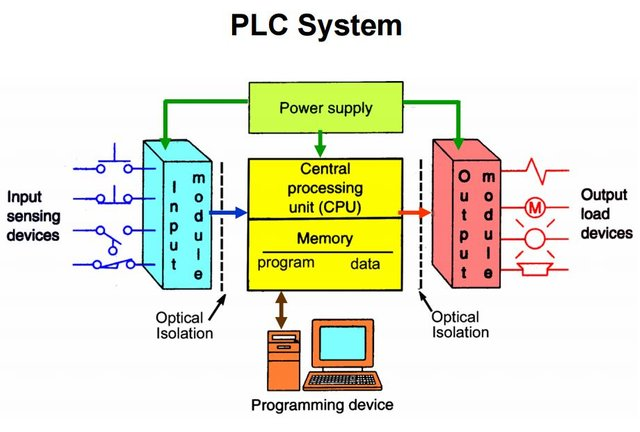
\includegraphics[ clip, trim=0.1cm 0.5cm 0.1cm 0.5cm, width=0.70\textwidth]{./images/plc.JPG}	\caption[Blockdiagramm SPS]{Blockdiagramm SPS\cite{URL:PLC}}
	\label{fig:plcFigure}
\end{figure}

%\subsection{Konzept?}
\subsection{Ausgangssituation} \label{chp:grundl:ausgangss}

Als Vorbild für dieses Projekt dient die Kleinsteuerung Easy vom Hersteller Eaton. Das Einstiegsmodell bietet acht Ein- und vier Ausgänge. Das Logikprogramm, welches die Eingänge der Steuerung logisch mit den Ausgängen verbindet, wird auf einem kleinen Display direkt am Gerät erstellt\cite{BOOK:Kleinsteuerungen}. Dabei stehen neben den physikalischen Ein- und Ausgängen auch Zeitfunktionen oder Zählerbausteine zur Verfügung. Im Programmiermodus, welcher in \autoref{fig:easyprogram} dargestellt ist, wird links ein Pluspol und rechts ein Minuspol symbolisiert. Der anzusteuernde Ausgang steht dabei stets ganz rechts. Der Strompfad kann nunmehr bis zum Pluspol durch gezeichnet, oder aber durch Sensoren unterbrochen und verzweigt werden. Aus diesem Schaltplan werden dann die booleschen Gleichungen gewonnen, welche die Steuerung im Betrieb durchläuft, um die Werte der Ausgänge zu bestimmen.

\begin{figure}[H]
	\centering
	\includegraphics[page=2, clip, trim=2.5cm 20cm 6.9cm 2.5cm, width=1.00\textwidth]{./code/GartenEasy.pdf}
	\caption{Programm einer Easy Kleinsteuerung}
	\label{fig:easyprogram}
\end{figure}

\subsubsection{Benutzeroberfläche} \label{kap:grundl:bedienoberfl}
Eine ähnliche Vorgehensweise bei der Erstellung des Logikprogramms (siehe \autoref{chp:grundl:ausgangss}) ist auch in diesem Projekt geplant. Da der Raspberry Pi netzwerkfähig ist, wurde jedoch statt eines Displays am Gerät eine Benutzeroberfläche gewählt, welche im Internetbrowser bedienbar ist. Als Basis für die Programmieroberfläche wurde das Projekt CircuitVerse\cite{URL:CircuitVerse} (siehe \autoref{kap:circuitVerse}) herangezogen. Hierbei handelt es sich um einen Logiksimulator, in welchem komplexe Logikschaltungen durch Drag\&Drop erstellt werden können. Das quelloffene Projekt ist auf GitHub\cite{URL:CircuitVerseGit} verfügbar und dank der MIT Lizenz zur Erweiterung und Modifikation freigegeben. Dabei musste das Projekt vor allem durch eine Funktion ergänzt werden, um die erstellte Logik in einem Format zu exportieren, welche vom Backend verstanden wird. Weiterhin mussten die zur Verfügung stehenden Bauteile dahingehend modifiziert werden, dass nur Schaltungen erstellt werden können, die auch im Backend implementiert sind. 
Im Vorbild der Easy Kleinsteuerung kann der Schaltplan auch Laufzeitinformationen wiedergeben. So wird ein (symbolisch) unter Spannung stehender Zweig als breite Linie dargestellt, während unbestromte Zweige schmal gezeichnet werden. Diese Laufzeitinformationen sollen in dieser Bachelorarbeit ebenfalls dargestellt werden. Dazu wird für jeden Ein- und Ausgang eine Grafik eingeblendet, welche erkennen lässt, ob der Eingang bzw. der Ausgang an oder aus ist.
\subsubsection{Backend} \label{chp:grundl:backend}
Als Schnittstelle zwischen Hardware und Bedienoberfläche wird eine Software eingesetzt, die das vom Benutzer erstellte Logikprogramm kontinuierlich durchläuft und somit sicherstellt, dass eine Änderung an einem Eingang, der Ablauf eines Timers etc. die Werte der davon abhängigen Ausgänge entsprechend verändert. Wie dies im Vorbild der Easy Kleinsteuerung gelöst wird, besteht kein Einblick.  

\subsubsection{Hardware}\label{chp:gundl:hardware}
Wie schon vorab beschrieben, bildet ein Raspberry Pi die Grundlage für dieses Projekt. Dieser bietet von Haus aus einige GPIOs, welche  dazu  verwendet werden können, um Sensoren abzufragen oder um Aktoren anzusteuern. Jedoch fiel die Entscheidung darauf, eine Erweiterungskarte (HAT) zu diesem Zweck einzusetzen. Dies dient zunächst zum Schutz des Raspberry Pi, zudem bietet die eingesetzte Erweiterungskarte auch Leuchtdioden an den Ausgängen sowie Taster an den Eingängen, was das Testen erheblich vereinfacht. Da der Anschluss per SPI erfolgt, können theoretisch mehrere solcher Boards parallel betrieben werden. Dies wird jedoch dadurch verhindert, dass die Erweiterungskarte die verwendeten Anschlüsse abdeckt. Ein Adaptermodul, welches die Anschlüsse vervielfacht, findet sich zwar im Internet, ist jedoch nicht mehr erhältlich. 

\subsection{Versionsverwaltung}
Da eine Versionsverwaltung für ein Projekt dieser Größe als notwendig erachtet wurde, fiel der Gedanke auf GIT.\cite{URL:GIT} Git ist eine dezentrale Versionsverwaltung, die Notwendigkeit eines Versionierungsservers entfällt hierdurch. Jedoch ist es in Git möglich, ein oder mehrere sogenannte Remotes hinzuzufügen. Das sind entfernte Git-Repositorys, die mit dem lokalen Repository synchronisiert werden können. In der Praxis wird Git häufig eingesetzt, weshalb sich diese Bachelorarbeit als Einarbeitung anbot. Zunächst wurde ein lokales Git Repository erstellt, welches in Folge mit einem Remote-Repository auf GitHub verbunden wurde. Angedacht war ein Development-Branch und jeweils ein Feature-Branch, welches nach Vollendung des entsprechenden Features in den Development-Branch zurückgeführt werden soll. Darüber hinaus soll ein Tagging erfolgen. Dabei soll für jeden Zeitbalken des Gantt Diagramms, welches in der vorhergehenden Projektplanung erstellt wurde, ein Tag gesetzt werden. 

\subsection{Entwicklungsumgebung}
Ein Problem, das dieses Projekt bietet, ist, dass nicht direkt auf dem Zielsystem entwickelt wird. Das hat zur Folge, dass das Programm entweder auf dem Entwicklungssystem crosskompiliert werden muss, oder die Quelldateien auf das Zielsystem kopiert werden müssen, um sie dort zu kompilieren. Da das Aufsetzen eines Crosskompilers inklusive der dazu nötigen Toolchain als zu aufwändig erachtet wurde, blieb nur der Weg, das Projekt direkt auf dem Zielsystem zu übersetzen. Um sich die Arbeit zu erleichtern, wurde nach einer Entwicklungsumgebung recherchiert, die ein Übersetzen über eine SSH Verbindung zulässt. NetBeans\cite{URL:NetBeans} bietet dies an, dabei wird entweder das gesamte Projekt beim Übersetzen per SSH auf das Zielsystem kopiert und dort übersetzt, oder es kann ein Ordner angegeben werden, an den eine Systemfreigabe eingehängt ist (z.B. über eine Samba-Freigabe). Im Laufe des Projektes wurde eigens dafür ein Samba-Server auf dem Zielsystem installiert. Von nun an konnte also in der Entwicklungsumgebung direkt auf den Dateien des Raspberry Pi gearbeitet werden, wobei per Tastendruck eine SSH Verbindung aufgebaut wurde, um auf dem Zielsystem den Befehl \chphl{make} auszuführen. Dabei werden sämtliche Ausgaben des Compilers in einem Fenster innerhalb der Entwicklungsumgebung angezeigt. Auch Debugging ist auf diesem Wege möglich.

\subsection{C++ Library LibPiFace}
Wie im Abschnitt \ref{chp:gundl:hardware} beschrieben, bildet die Erweiterungskarte PiFace Digital 2\cite{URL:PiFaceDigital2} die Grundlage für diese Bachelorarbeit. Im Lieferumfang befindet sich eine in C geschriebene Bibliothek inklusive eines lauffähigen Tests, welcher ebenfalls auf GitHub\cite{URL:PiFaceDigital2GIT} zu finden ist. Diese Bibliothek stützt sich wiederum auf die Bibliothek libmcp23s17\cite{URL:libmcp23s17}, welche den verbauten SoC über SPI anspricht. Im Laufe der Arbeiten fiel jedoch auf, dass die C Bibliothek nicht alle benötigten Funktionen enthielt. Da der Quellcode vorlag und die Lizenzierung Veränderungen am Quellcode zulässt, lag die Überlegung nahe, die benötigten Funktionen direkt in der Bibliothek zu ergänzen anstatt sie im eigentlichen Projekt unterzubringen. Weiterhin schien es auch ein erstrebenswertes Lernziel zu sein, das Erstellen und Übersetzen von statisch bzw. dynamisch gelinkten Bibliotheken kennenzulernen. Zuletzt wurde es schlichtweg als die sauberste Lösung erachtet. Zunächst wurde angenommen, dass sich auch mehrere Hardwaremodule per SPI mit einem einzelnen Raspberry Pi verbinden lassen. Dies ist technisch auch möglich, so bieten die eingesetzten Boards die Möglichkeit, über einen Jumper eine Hardwareadresse einzustellen. Der Hersteller bot auch die passende Hardware an, um mehrere Boards mit einem Raspberry Pi zu verbinden. Jedoch wurden diese scheinbar mangels Nachfrage aus dem Sortiment genommen. Obwohl eine Bastellösung es immer noch ermöglichen würde, ist der Aufwand hierfür sehr hoch und scheint unwirtschaftlich. Leider wurde bis zu dieser Erkenntnis schon einiges an Energie hinein investiert, mehrere Boards gleichzeitig zu unterstützen. Dies ist auch der ursprüngliche Grund, wieso ein objektorientierter Ansatz in C++ gewählt wurde - eine Instanz für jedes Hardware-Modul. Ein weiterer Grund war, dass die Anwendung ohne Caching nicht performant genug war. Das heißt, die zeitliche Lücke zwischen einer Änderung an einem Eingang bis zu dessen Auswirkung am Ausgang war deutlich spürbar und damit inakzeptabel. Dafür wurden Methoden vorgesehen, um das Caching ein- und auszuschalten - bei eingeschaltetem Caching verändern die Methoden, Bytes und Bits zu schreiben, lediglich den Wert einer Instanzvariable. Derzeit muss das Leeren des Caches explizit mit einem Aufruf der Methode \textit{flush()} erfolgen. Über ein automatisches Verfahren wurde nachgedacht, jedoch erwies sich der manuelle Aufruf als einfacher. 

\subsection{WebSocket} \label{chp:grdlgn:webSocket}
Damit die in \ref{kap:grundl:bedienoberfl} beschriebene Benutzeroberfläche Statusinformationen von der Steuerung erhalten kann, muss ein Kommunikationskanal zwischen dem Internetbrowser des Anwenders und der Steuerung geschaffen werden. Eine Kommunikation per HTTP ist dabei jedoch wenig flexibel, da dieses Protokoll zustandslos ist. Das bedeutet, dass eine Verbindung nach Bearbeitung einer Anfrage sofort wieder abgebaut wird. Es ist also per se nicht möglich, dass der Server den Client beim Eintreffen neuer Daten benachrichtigt. Eine Lösung hierfür wäre, die Anwendung im Browser so zu schreiben, dass sie den Server zyklisch anfragt. Dabei muss ein Kompromiss aus Serverbelastung, also kleinen Abfrageintervallen, und einer annehmbaren Verzögerung gefunden werden. Eine Verbesserung bringt \texttt{Long-Polling}. Hierbei wird auf Clientseite auf die gleiche Weise vorgegangen, der Server blockiert jedoch Anfragen bis zur maximalen Zeit eines Timeouts. Erhält der Client bis zum Timeout keine Daten, so stellt er nach dem Timeout erneut eine Anfrage. Bei diesen Methoden ist die Serverbelastung relativ hoch und beinhaltet eine gewisse Latenz, wodurch Anwendungen weniger schnell auf Änderungen reagieren können. WebSockets\cite{BOOK:Websockets} hingegen ermöglichen eine bidirektionale Kommunikation zwischen Server und Client, wobei die Latenz minimal ist. Dies begründet sich unter anderem dadurch, dass eine WebSocket-Verbindung persistent ist. Das heißt, sie wird einmalig aufgebaut und bleibt dann bestehen bis eine Seite die Verbindung beendet. Dadurch sind nur zum Aufbau der Verbindung Header nötig, was die zu übermittelnde Datenmenge drastisch reduziert. In der Praxis besteht ein HTTP Header, welcher jeder Anfrage mitgegeben werden muss, oft aus mehr als 100 Bytes. Eine WebSocket-Anfrage benötigt einen ebenso großen Header, jedoch nur um die Verbindung aufzubauen. Ist diese hergestellt, so werden lediglich zwei Byte je Übertragung fällig, um die Verbindung zu steuern. Das steigert nicht nur die Verbindungsgeschwindigkeit, sondern entlastet gleichzeitig den Server.\cite{URL:WebSocketOrg}


\subsection{Installation von Abhängigkeiten}\label{kap:ums:abh}
Wie sich im Laufe des Projektes herausstellte, benötigten einige Programmteile Funktionen aus der Boost-Bibliothek.\cite{BOOK:BOOST} Auf dem Desktop-Computer, auf dem die Lösung getestet wurde, konnte das Projekt dank installiertem Boost-Paket ohne Probleme übersetzt werden. Da es sich bei dem Zielsystem jedoch um eine ARM Architektur handelt, musste der Programmcode dort Übersetzt werden. In den Paketquellen des dort installieren Raspbian ist jedoch eine ältere Version des Boost-Pakets hinterlegt, was dazu führt, dass Boost manuell heruntergeladen und gebaut werden muss. Obwohl sich dieses Problem im Laufe der Zeit durch Aktualisierung des Paketes in den Paketquellen von Raspbian von selbst lösen wird, muss dennoch geprüft werden, ob die installierte Version den Ansprüchen genügt. Hierfür wurde ein Bash-Script erstellt, welches auch alle weiteren Abhängigkeiten prüft und gegebenenfalls installiert. Dazu zählen auch die im  \autoref{chp:anhang} \nameref{chp:anhang} aufgeführten Bibliotheken, um die Hardware anzusprechen, und der verwendete Kompiler. 

\clearpage


